\documentclass[border=10pt]{standalone}
\usepackage{pgfplots}
\pgfplotsset{compat=1.18}
\begin{document}
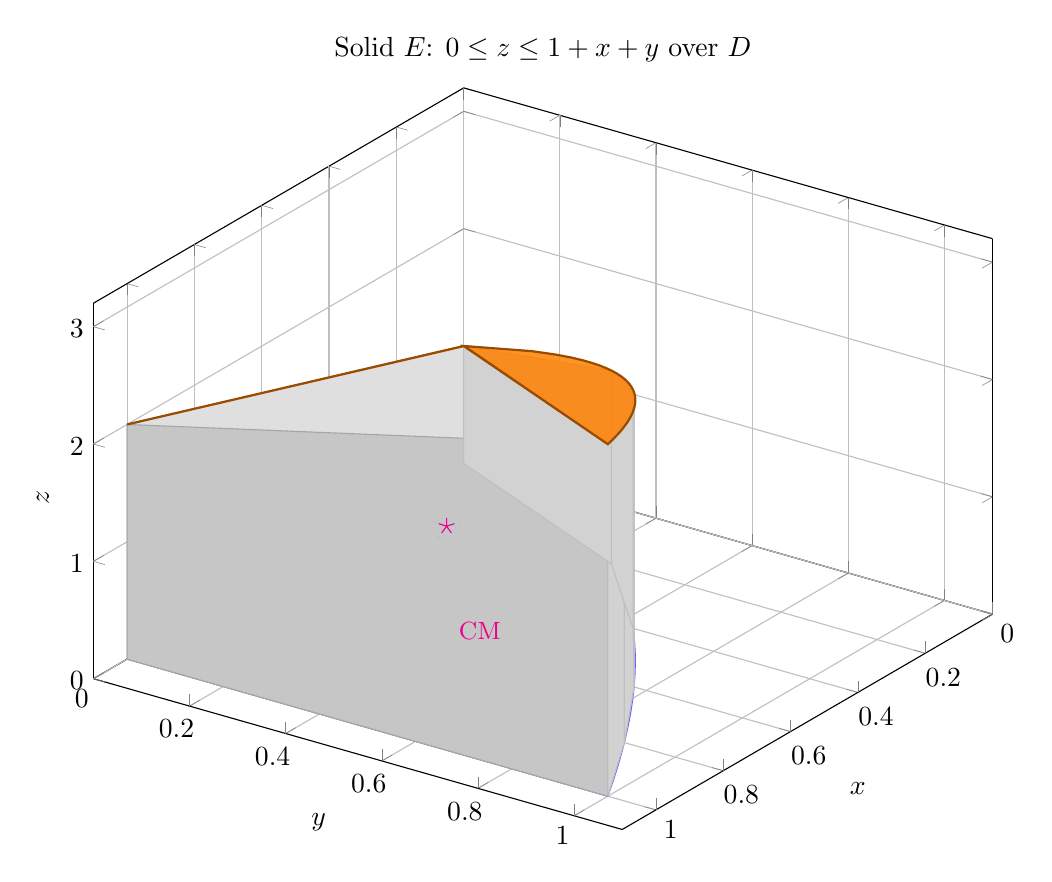
\begin{tikzpicture}
\begin{axis}[
    width=13cm, height=11cm,
    xlabel={$x$}, ylabel={$y$}, zlabel={$z$},
    xmin=0, xmax=1.1, ymin=0, ymax=1.1, zmin=0, zmax=3.2,
    view={125}{35},
    grid=major,
    title={Solid $E$: $0\leq z\leq 1+x+y$ over $D$},
]
% ---- bottom face: region D at z=0 (parabola boundary) ----
\addplot3[domain=0:1, samples=30, draw=blue!60, fill=blue, fill opacity=0.3]
    ({x}, {sqrt(x)}, 0) -- (axis cs:1,0,0) -- (axis cs:0,0,0) -- cycle;
% ---- back wall y=0: quad (0,0,0)-(1,0,0)-(1,0,2)-(0,0,1) ----
\addplot3[draw=gray!70, fill=gray!25] coordinates {(0,0,0) (1,0,0) (1,0,2) (0,0,1) (0,0,0)};
% ---- right wall x=1: quad (1,0,0)-(1,1,0)-(1,1,3)-(1,0,2) ----
\addplot3[draw=gray!70, fill=gray!45] coordinates {(1,0,0) (1,1,0) (1,1,3) (1,0,2) (1,0,0)};
% ---- curved wall y=sqrt(x): strips between x-levels (drawn back-to-front) ----
\addplot3[draw=gray!50, fill=gray!35] coordinates {(1,1,0) (0.8,0.8944,0) (0.8,0.8944,2.6944) (1,1,3) (1,1,0)};
\addplot3[draw=gray!50, fill=gray!35] coordinates {(0.8,0.8944,0) (0.6,0.7746,0) (0.6,0.7746,2.3746) (0.8,0.8944,2.6944) (0.8,0.8944,0)};
\addplot3[draw=gray!50, fill=gray!35] coordinates {(0.6,0.7746,0) (0.4,0.6325,0) (0.4,0.6325,2.0325) (0.6,0.7746,2.3746) (0.6,0.7746,0)};
\addplot3[draw=gray!50, fill=gray!35] coordinates {(0.4,0.6325,0) (0.2,0.4472,0) (0.2,0.4472,1.6472) (0.4,0.6325,2.0325) (0.4,0.6325,0)};
\addplot3[draw=gray!50, fill=gray!35] coordinates {(0.2,0.4472,0) (0,0,0) (0,0,1) (0.2,0.4472,1.6472) (0.2,0.4472,0)};
% ---- top face: planar region z = 1+x+y (drawn last, on top) ----
\addplot3[domain=1:0, samples=40, draw=orange!60!black, thick, fill=orange, fill opacity=0.85]
    ({x}, {sqrt(x)}, {1+x+sqrt(x)}) -- (axis cs:1,0,2) -- (axis cs:0,0,1) -- cycle;
% ---- center of mass ----
\addplot3+[only marks, mark=star, mark size=5pt, mark options={color=magenta, fill=magenta}] coordinates {(0.6474, 0.4177, 1.0325)};
\node[magenta, font=\small] at (axis cs:0.78, 0.58, 0.55) {CM};
\end{axis}
\end{tikzpicture}
\end{document}